\documentclass[crop=false]{standalone}
%\documentclass{standalone}
\usepackage{tikz} % To generate the plot from csv
\usepackage{pgfplots}
\usepackage{graphicx}
\usepackage{booktabs}
\usepackage{subfig}
\usepackage{float}
\usepackage[section]{placeins} % getting figures below sections
\usepackage{blindtext}
\usepackage{siunitx}
\usepgfplotslibrary{units} % Allows to enter the units nicely
\usetikzlibrary{external} %https://tex.stackexchange.com/questions/1460/script-to-automate-externalizing-tikz-graphics
\tikzexternalize[prefix=savedfigures/]

\pgfplotsset{compat=newest} % Allows to place the legend below plot
\usepackage{pgfplotstable}
\usepgfplotslibrary{statistics}

% #################### Function definition for box plots read table ##################\
\makeatletter
\pgfplotsset{
	boxplot prepared from table/.code={
		\def\tikz@plot@handler{\pgfplotsplothandlerboxplotprepared}%
		\pgfplotsset{
			/pgfplots/boxplot prepared from table/.cd,
			#1,
		}
	},
	/pgfplots/boxplot prepared from table/.cd,
	table/.code={\pgfplotstablecopy{#1}\to\boxplot@datatable},
	row/.initial=0,
	make style readable from table/.style={
		#1/.code={
			\pgfplotstablegetelem{\pgfkeysvalueof{/pgfplots/boxplot prepared from table/row}}{##1}\of\boxplot@datatable
			\pgfplotsset{boxplot/#1/.expand once={\pgfplotsretval}}
		}
	},
	make style readable from table=lower whisker,
	make style readable from table=upper whisker,
	make style readable from table=lower quartile,
	make style readable from table=upper quartile,
	make style readable from table=median,
	make style readable from table=average,
	make style readable from table=lower notch,
	make style readable from table=upper notch
}
\makeatother
\begin{document}

\section{24 1 Mandl6 SA Mutations more 20210817 144231}

% ######################## UTRP SA Mutation operators applied ######################## 
\begin{figure} 
\centering 
\tikzsetnextfilename{UTRP_DBMOSA_BP_mutation_funcs_more} 
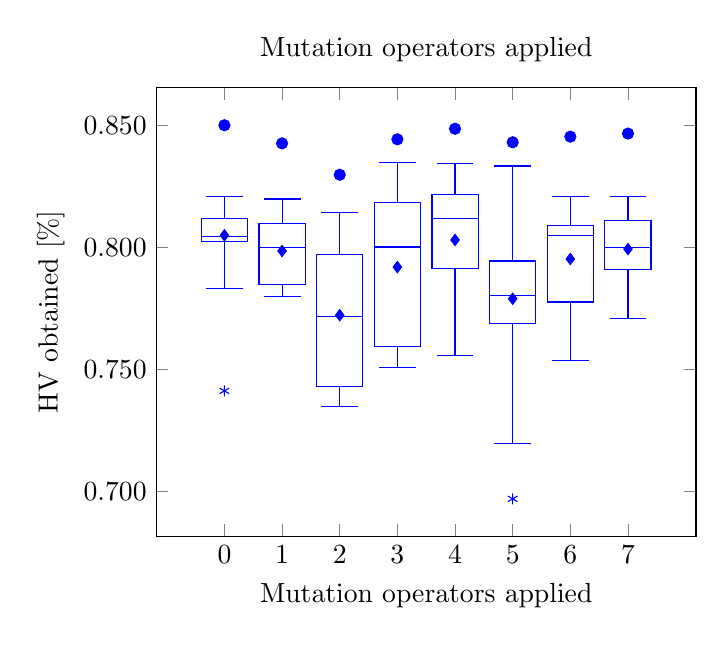
\begin{tikzpicture} 
\begin{axis}[ 
title={Mutation operators applied}, 
boxplot/draw direction=y, 
xtick={1,2,3,4,5,6,7,8}, 
xticklabels={0,1,2,3,4,5,6,7}, 
x tick label style={rotate=0, align=center}, 
xlabel={Mutation operators applied}, 
y tick label style={/pgf/number format/.cd,fixed,precision=3, zerofill}, 
ylabel={HV obtained [\%]}, 
] 

% ############## Mutations_more=0 ################## 
\addplot[boxplot, mark=asterisk, 
boxplot prepared={ 
lower whisker=0.78311, 
upper whisker=0.82093, 
lower quartile=0.80254, 
upper quartile=0.8119, 
median=0.80469, 
average=0.80503}, 
color = blue, solid, area legend] 
coordinates {
(1,0.7412)}; 
\addplot[only marks,mark=*,color = blue]coordinates{(1,0.85018)}; 

% ############## Mutations_more=1 ################## 
\addplot[boxplot, mark=asterisk, 
boxplot prepared={ 
lower whisker=0.77974, 
upper whisker=0.81991, 
lower quartile=0.78491, 
upper quartile=0.81004, 
median=0.79998, 
average=0.79857}, 
color = blue, solid, area legend] 
coordinates {}; 
\addplot[only marks,mark=*,color = blue]coordinates{(2,0.84274)}; 

% ############## Mutations_more=2 ################## 
\addplot[boxplot, mark=asterisk, 
boxplot prepared={ 
lower whisker=0.73482, 
upper whisker=0.81452, 
lower quartile=0.74301, 
upper quartile=0.79715, 
median=0.77166, 
average=0.77223}, 
color = blue, solid, area legend] 
coordinates {}; 
\addplot[only marks,mark=*,color = blue]coordinates{(3,0.82986)}; 

% ############## Mutations_more=3 ################## 
\addplot[boxplot, mark=asterisk, 
boxplot prepared={ 
lower whisker=0.75066, 
upper whisker=0.83474, 
lower quartile=0.75952, 
upper quartile=0.8183, 
median=0.80021, 
average=0.79198}, 
color = blue, solid, area legend] 
coordinates {}; 
\addplot[only marks,mark=*,color = blue]coordinates{(4,0.8444)}; 

% ############## Mutations_more=4 ################## 
\addplot[boxplot, mark=asterisk, 
boxplot prepared={ 
lower whisker=0.75562, 
upper whisker=0.83452, 
lower quartile=0.7915, 
upper quartile=0.82186, 
median=0.81201, 
average=0.80311}, 
color = blue, solid, area legend] 
coordinates {}; 
\addplot[only marks,mark=*,color = blue]coordinates{(5,0.84874)}; 

% ############## Mutations_more=5 ################## 
\addplot[boxplot, mark=asterisk, 
boxplot prepared={ 
lower whisker=0.7195, 
upper whisker=0.83345, 
lower quartile=0.7688, 
upper quartile=0.7945, 
median=0.78023, 
average=0.77899}, 
color = blue, solid, area legend] 
coordinates {
(6,0.6969)}; 
\addplot[only marks,mark=*,color = blue]coordinates{(6,0.84319)}; 

% ############## Mutations_more=6 ################## 
\addplot[boxplot, mark=asterisk, 
boxplot prepared={ 
lower whisker=0.75348, 
upper whisker=0.82108, 
lower quartile=0.77765, 
upper quartile=0.80906, 
median=0.80486, 
average=0.7953}, 
color = blue, solid, area legend] 
coordinates {}; 
\addplot[only marks,mark=*,color = blue]coordinates{(7,0.84549)}; 

% ############## Mutations_more=7 ################## 
\addplot[boxplot, mark=asterisk, 
boxplot prepared={ 
lower whisker=0.77074, 
upper whisker=0.82089, 
lower quartile=0.79093, 
upper quartile=0.81106, 
median=0.8002, 
average=0.79938}, 
color = blue, solid, area legend] 
coordinates {}; 
\addplot[only marks,mark=*,color = blue]coordinates{(8,0.84676)}; 

\end{axis}
\end{tikzpicture}
\end{figure} 
\begin{table}
\centering
\caption{Legend for the boxplot.}
\begin{tabular}{ll}
\toprule
 Index &                                               Name \\
\midrule
     0 & [Add\_vertex, Delete\_vertex, Insert\_inside\_verte... \\
     1 & [MSC\_add\_terminal, MSC\_del\_terminal, Insert\_ins... \\
     2 & [Trim\_one\_terminal\_cb, Grow\_one\_terminal\_cb, In... \\
     3 & [Intertwine\_two, Add\_vertex, Delete\_vertex, Inv... \\
     4 & [Intertwine\_two, MSC\_add\_terminal, MSC\_del\_term... \\
     5 & [Intertwine\_two, Trim\_one\_terminal\_cb, Grow\_one... \\
     6 & [Intertwine\_two, Add\_vertex, Delete\_vertex, Inv... \\
     7 & [Intertwine\_two, MSC\_add\_terminal, MSC\_del\_term... \\
\bottomrule
\end{tabular}
\end{table}

\end{document}
